\documentclass[letterpaper,12pt,fleqn]{article}
\usepackage{matharticle}
\usepackage{siunitx}
\renewcommand{\o}{\theta}
\pagestyle{plain}
\begin{document}

\begin{center}
\Large Math-19 Homework \#15 Solutions
\end{center}

\vspace{0.5in}

\underline{Problems}

\begin{enumerate}

\item Consider the function:
  \[f(x)=2\tan(4\pi x-\pi)+1=
  2\tan\left[4\pi\left(x-\frac{1}{4}\right)\right]+1\]
  \begin{enumerate}
  \item What is the period $P$?
    \[P=\frac{\pi}{4\pi}=\frac{1}{4}\]
    
  \item What is the horizontal translation $b$?
    \[\frac{1}{4}\ \mbox{to the right}\]
    
  \item What is the phase angle $\phi$?
    \[\pi=-\pi\]
    
  \item What is the y-intercept?
    \[f(0)=2\tan(-\pi)+1=0+1=1\]
    $(0,1)$
    
  \item Sketch one cycle of the graph in the interval
    $\left(b+\frac{P}{2},b-\frac{P}{2}\right)$ and then extend the sketch back
    to the y-intercept.

    \begin{tikzpicture}
      \draw (-1,0) -- (4,0);
      \draw (0,-4) -- (0,4);
      \draw [dashed] (-1,1) -- (4,1);
      \draw [dashed] (1,-4) -- (1,4);
      \draw [dashed] (3,-4) -- (3,4);
      \draw [dashed] (2,0) -- (2,1);
      \node [above left] at (0,1) {$1$};
      \node [below left] at (1,0) {$\frac{1}{8}$};
      \node [below] at (2,0) {$\frac{1}{4}$};
      \node [below right] at (3,0) {$\frac{3}{8}$};
      \draw [smooth,domain=1.28:2.65] plot ({\x},{2*tan(pi/2*(\x*180/pi-2))+1});
      \draw [smooth,domain=0:0.65] plot ({\x},{2*tan(pi/2*(\x*180/pi-2))+1});
    \end{tikzpicture}
  \end{enumerate}

\item Two $\SI{1}{kg}$ masses are each suspended on a spring with $k=\pi^2$ and
  are stretched downward by 2 units. The first spring is released at $t=0$. The
  second spring is released at $t=3$.
  \begin{enumerate}
  \item Find $f_1(t)$ for the first mass.
    \[f_1(t)=2\cos\left(\sqrt{\frac{\pi^2}{1}}t\right)=2\cos\pi t\]
    
  \item Find $f_2(t)$ for the second mass.
    \[f_2(t)=2\cos\pi(t-3)=2\cos(\pi t-3\pi)\]
    
  \item What is the phase difference between the two masses?
    The phase angle in the previous part is $3\pi$; however, since the period is
    only $2\pi$, we can state the phase angle as $3\pi-2\pi=\pi$ or
    $180^{\circ}$.
  \end{enumerate}

\item Evaluate:
  \[\cot\left(\cos^{-1}\frac{x}{\sqrt{1+x^2}}\right)\]

  First, we repeat to ourselves, ``the angle whose cosine is ....'' Next, we
  draw a right triangle corresponding to our angle:

  \begin{figure}[h]
  \setlength{\leftskip}{1in}
  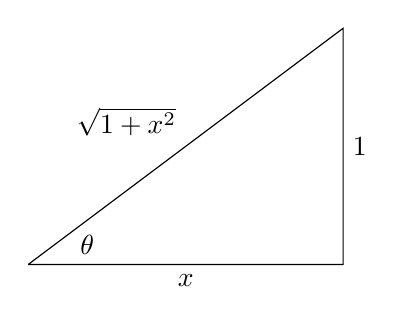
\begin{tikzpicture}
    \draw (0,0) -- (4,0) -- (4,3) -- (0,0);
    \node at (0.75,0.25) {$\o$};
    \node [below] at (2,0) {$x$};
    \node [right] at (4,1.5) {$1$};
    \node [above left] at (2,1.5) {$\sqrt{1+x^2}$};
  \end{tikzpicture}
  \end{figure}

  Note that by using the Pythagorean theorem we determine that the length of
  the opposite side is 1.  We now take the cotangent of our angle:
  \[\cot\left(\cos^{-1}\frac{x}{\sqrt{1+x^2}}\right)=\frac{x}{1}=x\]

\item A water tower is located $\SI{500}{ft}$ from a building. An observer
  looks at the tower from a window in the building. The angle of depression
  to the bottom of the tower is $45^{\circ}$. The angle of elevation to the
  top of the tower is $15^{\circ}$. How tall is the tower (to the nearest foot)?

  \begin{center}
    \begin{tikzpicture}
      \node [draw,circle,fill,scale=0.5] (w) at (0,0) {};
      \node [draw,circle,fill,scale=0.5] (t) at (5,5) {};
      \node [draw,circle,fill,scale=0.5] (b) at (5,-1) {};
      \draw (b) to node [right] {$h_1$} (5,0);
      \draw (5,0) to node [right] {$h_2$} (t);
      \draw [dashed] (w) to (t);
      \draw [dashed] (w) to (b);
      \draw [dashed] (w) to node [above] {$\SI{500}{ft}$} (5,0);
      \node at (0.75,0.3) {$45^{\circ}$};
      \node at (2,-0.25) {$15^{\circ}$};
    \end{tikzpicture}
  \end{center}

  $\tan(15^{\circ})=\frac{h_1}{500}$ and so $h_1=500\tan(15^{\circ})$.

  $\tan(45^{\circ})=\frac{h_2}{500}$ and so $h_2=500\tan(45^{\circ})$.

  $h=h_1+h_2=500[\tan(15^{\circ})+\tan(45^{\circ})]\approx\SI{634}{ft}$
\end{enumerate}
 
\end{document}
